% Publication figure generated from the actual reference and M1 runs.
% Required packages in the parent document:
%   \usepackage{graphicx}
%   \usepackage{subcaption}
%
% MATLAB source:
%   verification/crack_path/plot_m1_vs_reference_publication.m
%
% Generated vector panels:
%   trajectory.pdf
%   vertical_deviation.pdf
%   direction_deviation.pdf
%   mode_mixity.pdf

\begin{figure}[tbp]
  \centering

  \begin{subfigure}[t]{0.94\linewidth}
    \centering
    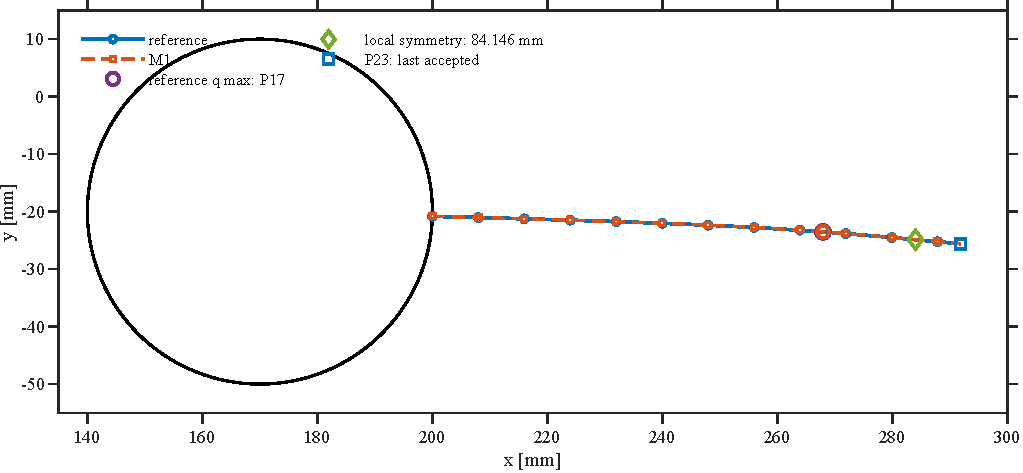
\includegraphics[width=\linewidth]{figures/m1_mesh_sensitivity/trajectory.pdf}
    \caption{Actual crack trajectories obtained with the reference exterior
    mesh and the independently propagated M1 exterior mesh. The two paths
    are visually indistinguishable at the scale of the specimen.}
    \label{fig:m1mesh-trajectory}
  \end{subfigure}

  \medskip

  \begin{subfigure}[t]{0.315\linewidth}
    \centering
    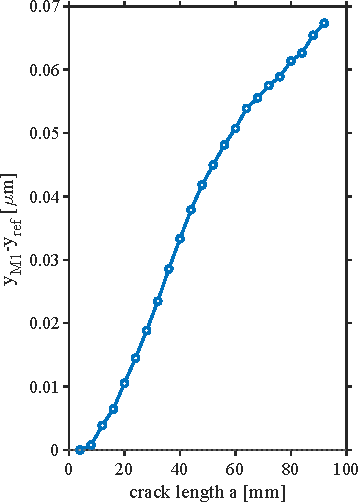
\includegraphics[width=\linewidth]{figures/m1_mesh_sensitivity/vertical_deviation.pdf}
    \caption{Accumulated vertical tip-coordinate difference,
    $y_{\mathrm{M1}}-y_{\mathrm{ref}}$.}
    \label{fig:m1mesh-dy}
  \end{subfigure}
  \hfill
  \begin{subfigure}[t]{0.315\linewidth}
    \centering
    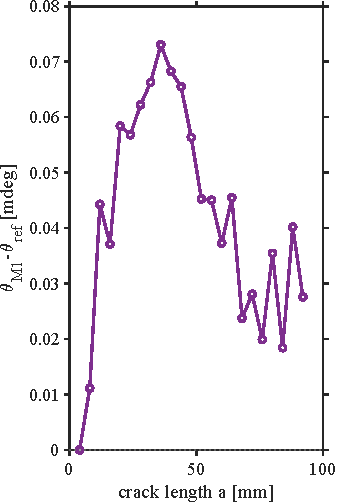
\includegraphics[width=\linewidth]{figures/m1_mesh_sensitivity/direction_deviation.pdf}
    \caption{Difference in the absolute crack direction in the frozen initiation frame,
    $\theta_{\mathrm{M1}}-\theta_{\mathrm{ref}}$.}
    \label{fig:m1mesh-dtheta}
  \end{subfigure}
  \hfill
  \begin{subfigure}[t]{0.315\linewidth}
    \centering
    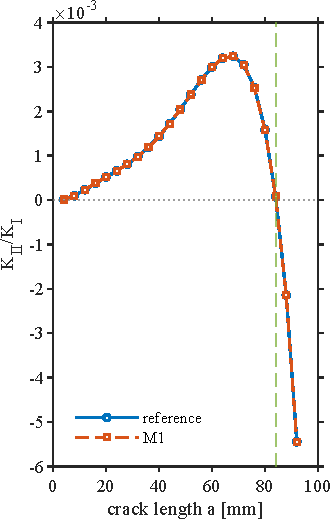
\includegraphics[width=\linewidth]{figures/m1_mesh_sensitivity/mode_mixity.pdf}
    \caption{Mode-mixity ratio $K_{II}/K_I$ along the two independently
    propagated trajectories.}
    \label{fig:m1mesh-q}
  \end{subfigure}

  \caption{Sensitivity of the incremental LEFM trajectory to coarsening of
  the exterior mesh. The M1 calculation retains the audited crack-tip core
  and EDI extraction region but uses a substantially coarser exterior mesh.
  The comparison is based on two independently propagated trajectories:
  the M1 calculation recomputes the $P_1$ SIFs and every subsequent MTS
  update rather than reusing the reference vertices.}
  \label{fig:m1-mesh-sensitivity}
\end{figure}
